\documentclass[runningheads]{llncs}
\usepackage{rotating,graphicx}
\usepackage{amsmath,amssymb}
\usepackage{booktabs,longtable,multirow}
\usepackage{float}
\usepackage{hyperref}
\usepackage{xcolor}
\usepackage{algorithm}
\usepackage{algorithmicx}

\setcounter{secnumdepth}{4}

\begin{document}

\title{Transformer-Based Fake News Detection: A Comparative Analysis of BERT, BiLSTM, and Hybrid Architectures Across Multiple Datasets}


\author{Md Akash Hossain\inst{1} and Parijata Majumdar \inst{2}}
\authorrunning{HOSSAIN, A. et al.}
\institute{Department of Information Technology, Tripura University, Tripura, India\\
\email{hossainakash22958@gmail.com} \and
\email{parijatamajumdar@tripurauniv.ac.in}
}

\maketitle              % typeset the header of the contribution

\begin{abstract}
The objective of fake news detection is to employ computing tools such as NLP and ML to identify and categorize fake or misleading information. The proliferation of misinformation through digital media channels poses threats to public perception, democratic governance, and information reliability, requiring automatic fake news detection systems that can handle large amounts of data.

In this paper, a layered model for fake news detection has been proposed that employs NLP for text preprocessing, feature extraction, and comparative analysis of multiple models. In the process of text preprocessing, noise reduction, tokenization, stopword elimination, and lemmatization are some of the processes applied to standardize textual information.

This paper analyzes three fundamental models such as BiLSTM, BERT, and BERT + BiLSTM models on various benchmark datasets, such as LIAR and ISOT for assessing generalization ability. From the experimental analysis, it can be seen that the standalone model of BiLSTM demonstrates relatively poor performance since it gives only 50\% accuracy rate, where its F1 score is equal to 0.3333. This can be explained by the fact that the model has been trained only for a few epochs without performing extensive hyperparameter tuning. On the other hand, the BERT model demonstrates a much better performance than any sequential models because it gives up to 95\% accuracy, where the precision equals 0.9545, while recall equals 0.9500.
The above results illustrate the efficiency of using transformer-based models in detecting fake news. The proposed system can be easily scalable and used for practical implementation in real-life scenarios like social media monitoring and fact-checking. Further research aims to incorporate large language models and explainable AI into the system.

\keywords{Fake news detection, Natural Language Processing, Machine Learning, Explainable AI, Misinformation.}
\end{abstract}

\section{Introduction}
\subsection{Background and Motivation}

The detection of fake news is basically an automated process that involves detecting and categorizing false, misleading, or fabricated information portrayed as true news by using advanced computational methods such as NLP and ML \cite{Shu2020FakeNewsNet,Shu2017FakeNewsDetection}. Due to the emergence of digital media platforms, there has been an increase in the amount of information being generated and transmitted online at an unprecedented rate.

Such an issue presents various challenges, including the manipulation of public perception, interference with democratic procedures, and erosion of confidence in reliable information sources \cite{Shu2020FakeNewsNet,Shu2017FakeNewsDetection}. Researches have demonstrated that lies and untruths spread quickly among social media sites as compared to the actual news \cite{Vosoughi2018Spread}. It is hard for reporters and fact-checkers to keep up with such a quick pace of spread and verify the news manually.

Furthermore, the spread of disinformation can have disastrous effects on the society and economy. Therefore, the development of such systems that are capable of detecting fake news automatically is an important research challenge.

\subsection{Types of Fake News}

The term fake news encompasses an amalgamation of news items belonging to distinct classes with varying motives and features. For instance, the five main types of fake news include:

\begin{itemize}
\item \textbf{False News Stories:} Fabricated information deliberately designed to deceive readers.
\item \textbf{Manipulated News:} Real information that has been manipulated or distorted in some way.
\item \textbf{Satirical News:} Ridiculous or hyperbolic news that may be taken seriously.
\item \textbf{Clickbait:} News stories with misleading titles.
\item \textbf{Propaganda:} Biased or misleading information aimed at shaping perceptions or advancing certain causes.
\end{itemize}

The diversity present in these categories leads to many difficulties that arise in the automatic detection process because of the unique characteristics possessed by these classes. Thus, there is a necessity to devise powerful models that can efficiently handle the meaning and contextual relationship within textual information.

\subsection{Role of Machine Learning and Deep Learning Methods}

Machine learning and deep learning techniques have been able to prove themselves effective when used to detect fake news because of the ability of these models to extract complicated patterns from large sets of data. There are classical machine learning algorithms like Logistic Regression, Support Vector Machine (SVM), Naive Bayes, and Random Forest.
Deep learning models such as LSTM and BiLSTM are built for identifying sequences within the text. Yet, their effectiveness may be undermined when complex associations between contexts are involved, especially with a limited amount of training data or inadequate training time.

Transformers like BERT (Bidirectional Encoder Representations from Transformers) have outperformed existing sequential models by generating bidirectional contextualized representation of text \cite{Kaliyar2021FakeBERT, Mehta2022RecentTrends}. While sequential models rely on a sequential approach to process texts, BERT considers the whole input context at once, thereby gaining insight into semantic relations.

The textual inputs are encoded numerically using methods like TF-IDF, bag-of-words, Word2Vec, GloVe, and BERT embedding. Such encoding allows models to learn discriminatory features for classification.

\subsection{Overview of the Proposed System}

The suggested fake news detection model is intended to work as a multi-stage processing pipeline where news input data will be received up until the process ends in detecting fake news and making a report of the results. The proposed model can handle various input types, like textual information, news headlines, and URLs to web pages containing news articles.

Training and testing the model are performed using well-known benchmark datasets like LIAR, ISOT, and FakeNewsNet. Benchmark datasets contain examples of both real and fake news data. The ability of the models to generalize and perform across multiple datasets is evaluated through testing and comparing their results on various datasets.

The model contains an NLP preprocessing step that involves cleaning and normalizing the news text data by performing tokenization, stop-word elimination, stemming, lemmatization, and lowercase transformations.

Text representation is performed in the feature extraction layer through techniques such as TF-IDF, Bag-of-Words, Word2Vec, GloVe, and BERT’s contextual embedding. Such transformations enable statistical as well as semantic properties of text to be captured effectively.

In terms of the classification layer, a variety of models were analyzed, namely, BiLSTM, BERT, and an ensemble of BERT + BiLSTM. Experiments indicate that the model based on BiLSTM obtains poor results compared to the others, and this might be due to a small number of training epochs, insufficient fine-tuning of the model, and a complicated nature of the used dataset. However, the BERT model provides superior performance since it makes use of pre-trained contextual embeddings. Interestingly, there is no significant difference between the results obtained from BERT and BERT + BiLSTM.

Finally, the output layer is responsible for labeling the input data as either \textit{real} or \textit{fake} news and producing corresponding confidence estimates. A reporting mechanism was introduced to generate comprehensible output.

\subsection{Contribution}

This study makes the following key contributions:

\begin{itemize}
\item Suggests an architecture for detecting fake news using a multi-level approach that combines natural language processing preprocessing, feature extraction, and classification techniques.
\item Compares different models including BiLSTM, BERT, and BERT with BiLSTM through various experiments on several datasets.
\item Shows the superiority of transformer models in the fake news detection task.
\item Investigates the drawbacks of sequential models and their hybrid models under restricted training conditions.
\item Indicates the promising areas for future research that focus on LLMs and XAI approaches.
\end{itemize}


\subsection{Paper Organization}
The rest of the paper is structured as follows. Section 2 provides an extensive literature review of related work on techniques used for detecting fake news using traditional machine learning techniques, deep learning algorithms, and transformers. Section 3 explains the proposed system design. Section 4 explains the methodology, experiment, dataset, and results. Section 5 concludes the paper and discusses future scope of work.

\section{Related Work}

In this section, we review nineteen peer-reviewed articles that form the basis of our research. The selected articles have been organized thematically, starting from traditional ML techniques, then moving on to deep learning and transformers. Finally, we discuss the role of explainability and LLMs. We have summarized all the articles in Table \ref{tab:litreview}.

\begin{longtable}{|p{0.19\textwidth}|p{0.19\textwidth}|p{0.18\textwidth}|p{0.18\textwidth}|p{0.18\textwidth}|}
\caption{Comparative Literature Review of Fake News Detection Methods} \label{tab:litreview} \\
\hline
\textbf{Contribution} & \textbf{Method} & \textbf{Advantage} & \textbf{Disadvantage} & \textbf{Future Scope} \\ \hline
\endfirsthead
\hline
\textbf{Contribution} & \textbf{Method} & \textbf{Advantage} & \textbf{Disadvantage} & \textbf{Future Scope} \\ \hline
\endhead
\hline
\multicolumn{5}{r}{\small\textit{Continued on next page\ldots}} \\
\endfoot
\hline
\endlastfoot
Introduced FakeBERT, a BERT-based deep learning model specifically designed for fake news detection on social media platforms with parallel CNN layers integrated into BERT architecture \cite{Kaliyar2021FakeBERT}. &
BERT + Parallel CNN layers for multi-scale feature extraction on LIAR and ISOT datasets \cite{Kaliyar2021FakeBERT}. &
Achieved 98.90\% accuracy; effectively captures contextual semantic relationships in text; outperforms traditional ML models significantly \cite{Kaliyar2021FakeBERT}. &
Computationally expensive; requires large GPU memory; limited to English language content only \cite{Kaliyar2021FakeBERT}. &
Extend to multilingual detection; reduce computational cost using model distillation techniques \cite{Kaliyar2021FakeBERT}. \\ \hline
Systematically compared multiple classical ML classifiers for fake news detection using linguistic and statistical text features extracted via TF-IDF \cite{Aphiwongsophon2021Detecting}. &
Logistic Regression, SVM, Naive Bayes, Random Forest with TF-IDF feature vectors on benchmark news datasets \cite{Aphiwongsophon2021Detecting}. &
Simple implementation; low computational cost; interpretable results; suitable for resource-constrained environments \cite{Aphiwongsophon2021Detecting}. &
Lower accuracy compared to deep learning; cannot capture semantic context or word order in text \cite{Aphiwongsophon2021Detecting}. &
Combine classical ML with deep learning features; incorporate metadata and social context signals \cite{Aphiwongsophon2021Detecting}. \\ \hline
Proposed a hybrid deep learning architecture combining CNN for local feature extraction and RNN for sequential pattern learning in news text \cite{Nasir2021FakeNews}. &
Hybrid CNN-RNN architecture with GloVe word embeddings trained on ISOT and FA-KES datasets \cite{Nasir2021FakeNews}. &
Captures both local and sequential text features simultaneously; better generalization than single-model approaches \cite{Nasir2021FakeNews}. &
Requires significant training data; slow inference time; struggles with short text like tweets and headlines \cite{Nasir2021FakeNews}. &
Apply to real-time social media streams; incorporate attention mechanisms for better interpretability \cite{Nasir2021FakeNews}. \\ \hline
Analyzed stylometric and linguistic style features that distinguish fake news from credible news using writing patterns and rhetorical structures \cite{Przybyla2020Capturing}. &
Stylometric analysis with SVM classifier; features include sentence length, punctuation patterns, readability scores on news datasets \cite{Przybyla2020Capturing}. &
Does not require external knowledge base; works purely on writing style; lightweight and fast inference \cite{Przybyla2020Capturing}. &
Style-based features are easily mimicked by sophisticated fake news creators; low robustness against adversarial content \cite{Przybyla2020Capturing}. &
Combine style features with semantic embeddings for more robust multi-feature detection systems \cite{Przybyla2020Capturing}. \\ \hline
Proposed evidence-aware fake news detection by retrieving external web evidence and combining it with claim credibility assessment using attention networks \cite{Popat2019DeClarE}. &
Attention-based LSTM with external web evidence retrieval and source credibility scoring on Snopes and PolitiFact datasets \cite{Popat2019DeClarE}. &
Incorporate external knowledge for verification; attention mechanism provides interpretability; better performance on political claims \cite{Popat2019DeClarE}. &
Dependent on external evidence availability; slow due to web retrieval; fails when evidence is unavailable or biased \cite{Popat2019DeClarE}. &
Integrate real-time knowledge graphs; improve evidence retrieval with more reliable fact-checking APIs \cite{Popat2019DeClarE}. \\ \hline
Developed a comprehensive fake news benchmark dataset incorporating news content, user social engagement, and spatiotemporal propagation features \cite{Shu2020FakeNewsNet}. &
Multi-modal dataset construction combining news text, social network graphs, user profiles, and publisher credibility on PolitiFact and GossipCop \cite{Shu2020FakeNewsNet}. &
Most comprehensive publicly available dataset; enables multi-modal detection research; includes social context signals \cite{Shu2020FakeNewsNet}. &
Dataset collection is time-consuming; social context features require platform API access which is increasingly restricted \cite{Shu2020FakeNewsNet}. &
Expand dataset to include video and image modalities; add multilingual fake news samples \cite{Shu2020FakeNewsNet}. \\ \hline
Surveyed state-of-the-art deep learning techniques for fake news detection covering transformer models, graph neural networks, and multi-modal approaches \cite{Mehta2022RecentTrends}. &
Systematic review of BERT, GPT, GNN, and multi-modal models across multiple benchmark datasets from 2017 to 2022 \cite{Mehta2022RecentTrends}. &
Comprehensive coverage of recent methods; identifies research gaps; provides clear taxonomy of detection approaches \cite{Mehta2022RecentTrends}. &
Survey only; no novel model proposed; coverage limited to English language studies \cite{Mehta2022RecentTrends}. &
Develop unified evaluation benchmark; explore cross-lingual and low-resource fake news detection \cite{Mehta2022RecentTrends}. \\ \hline
Combined BERT contextual embeddings with enhanced LSTM architecture for improved sequential and contextual understanding of fake news text \cite{Rai2022FakeNews}. &
BERT + enhanced LSTM hybrid model with attention mechanism trained on LIAR and ISOT datasets \cite{Rai2022FakeNews}. &
Superior performance over standalone BERT or LSTM; attention layer improves interpretability; robust to text length variations \cite{Rai2022FakeNews}. &
High model complexity; longer training time; requires substantial labeled data for effective fine-tuning \cite{Rai2022FakeNews}. &
Apply transfer learning to low-resource languages; integrate image features for multi-modal detection \cite{Rai2022FakeNews}. \\ \hline
Investigated psychological and cognitive bias patterns embedded in fake news content using computational linguistics and psycholinguistic feature analysis \cite{CarrascoFarre2022Fingerprints}. &
Psycholinguistic feature extraction using LIWC tool with ML classifiers; analysis of cognitive bias markers in fake vs.\ real news articles \cite{CarrascoFarre2022Fingerprints}. &
Novel perspective combining psychology and NLP; interpretable features; applicable across domains and languages \cite{CarrascoFarre2022Fingerprints}. &
Limited dataset size; psycholinguistic tools may not generalize across cultural and linguistic contexts \cite{CarrascoFarre2022Fingerprints}. &
Extend psycholinguistic analysis to social media posts; develop cross-cultural misinformation detection models \cite{CarrascoFarre2022Fingerprints}. \\ \hline
Proposed an optimized ensemble learning model using metaheuristic harmony search algorithm for automatic feature selection and classifier weight optimization \cite{Huang2020FakeNews}. &
Ensemble of SVM, RF, and LR optimized using Self-Adaptive Harmony Search metaheuristic algorithm on multiple news datasets \cite{Huang2020FakeNews}. &
Automatic feature selection reduces dimensionality; ensemble approach improves robustness; outperforms individual classifiers \cite{Huang2020FakeNews}. &
High computational overhead due to metaheuristic optimization; complex implementation; not suitable for real-time detection \cite{Huang2020FakeNews}. &
Apply neural architecture search for automated deep learning model optimization in fake news detection \cite{Huang2020FakeNews}. \\ \hline
Provided a foundational data mining perspective on fake news detection on social media, proposing taxonomy of detection methods including knowledge-based, style-based, propagation-based, and credibility-based approaches \cite{Shu2017FakeNewsDetection}. &
Survey and taxonomy of fake news detection approaches on social media platforms; analysis of linguistic, visual, and social context features \cite{Shu2017FakeNewsDetection}. &
Comprehensive taxonomy; covers diverse detection paradigms; foundational reference for the research community \cite{Shu2017FakeNewsDetection}. &
Survey only; no experimental results; limited coverage of deep learning and transformer-based models \cite{Shu2017FakeNewsDetection}. &
Develop end-to-end multi-modal systems combining all four detection paradigms for improved accuracy \cite{Shu2017FakeNewsDetection}. \\ \hline
Presented a comprehensive survey of fake news fundamental theories, detection methods, and future opportunities covering the full spectrum from fabrication to verification \cite{Zhou2020Survey}. &
Systematic review of knowledge-based, style-based, propagation-based, and credibility-based detection methods across multiple benchmark datasets \cite{Zhou2020Survey}. &
Thorough coverage of detection strategies; identifies open problems; provides structured framework for future research \cite{Zhou2020Survey}. &
Survey only; does not propose a novel detection model; limited coverage of multimodal and LLM-based approaches \cite{Zhou2020Survey}. &
Extend survey coverage to include graph neural networks, multimodal detection, and cross-lingual fake news models \cite{Zhou2020Survey}. \\ \hline
Proposed CSI (Capture, Score, Integrate), a hybrid deep learning model combining text content features with user behaviour and propagation patterns for fake news detection \cite{Ruchansky2017CSI}. &
Hybrid RNN model integrating article text (Capture), user response scoring, and propagation network modelling on CIKM benchmark dataset \cite{Ruchansky2017CSI}. &
First to integrate content, user, and propagation signals; significantly outperforms text-only baselines; applicable to social media platforms \cite{Ruchansky2017CSI}. &
Requires social engagement data which may be unavailable; complex multi-module architecture; limited generalization to non-social media news \cite{Ruchansky2017CSI}. &
Extend to real-time streaming data; integrate image and video modalities; explore graph-based propagation modelling \cite{Ruchansky2017CSI}. \\ \hline
Conducted a landmark empirical study on the spread of true and false news online across Twitter, revealing that false news spreads six times faster than true news and reaches more people \cite{Vosoughi2018Spread}. &
Large-scale analysis of 126,000 news stories tweeted by three million users over ten years; statistical modelling of diffusion cascades \cite{Vosoughi2018Spread}. &
Largest empirical study of its kind; provides strong motivation for automated fake news detection; highlights human-driven amplification of misinformation \cite{Vosoughi2018Spread}. &
Observational study; does not propose a detection model; limited to Twitter platform data \cite{Vosoughi2018Spread}. &
Extend analysis to other social media platforms; design detection systems that model propagation speed as a real-time detection signal \cite{Vosoughi2018Spread}. \\ \hline
Introduced the LIAR benchmark dataset containing 12,836 manually labelled short statements from PolitiFact with six fine-grained truthfulness labels for fake news detection research \cite{Wang2017Liar}. &
Benchmark dataset construction with metadata including speaker, subject, context, and party affiliation; baseline CNN and BiLSTM classifiers evaluated \cite{Wang2017Liar}. &
First large-scale manually labelled fake news dataset; enables fine-grained classification; metadata-rich annotations support multi-feature modelling \cite{Wang2017Liar}. &
Limited to political speech domain; fine-grained labels make classification harder; dataset may not generalize to social media news content \cite{Wang2017Liar}. &
Extend dataset with image and video evidence; develop cross-domain transfer learning models trained on LIAR for general fake news detection \cite{Wang2017Liar}. \\ \hline
Introduced LLaMA 2, a family of open-source large language models ranging from 7B to 70B parameters, enabling state-of-the-art language understanding and generation for downstream NLP tasks \cite{Touvron2023Llama2}. &
Open-source transformer-based LLM family fine-tuned for dialogue and instruction following; evaluated on multiple NLP benchmarks against GPT-4 and other proprietary models \cite{Touvron2023Llama2}. &
Freely available for research; competitive performance against closed models; enables privacy-preserving local deployment of large language models \cite{Touvron2023Llama2}. &
Requires significant GPU resources for inference and fine-tuning; may still produce hallucinations; limited multilingual capability compared to GPT-4 \cite{Touvron2023Llama2}. &
Fine-tune LLaMA 2 on fake news datasets; integrate with RAG pipelines to enable evidence-grounded fake news classification \cite{Touvron2023Llama2}. \\ \hline
Proposed Retrieval-Augmented Generation (RAG), a framework combining parametric knowledge of pre-trained LLMs with non-parametric retrieval from external knowledge bases for knowledge-intensive NLP tasks \cite{Lewis2020RAG}. &
RAG model combining dense passage retrieval with a sequence-to-sequence generator; evaluated on open-domain QA, fact verification, and knowledge-grounded dialogue tasks \cite{Lewis2020RAG}. &
Enables LLMs to access up-to-date external evidence; reduces hallucination; improves factual accuracy without full model retraining \cite{Lewis2020RAG}. &
Retrieval quality is highly dependent on the quality and coverage of the knowledge base; increased inference latency due to retrieval step \cite{Lewis2020RAG}. &
Apply RAG to fake news detection by grounding classification decisions in retrieved evidence from verified fact-checking databases \cite{Lewis2020RAG}. \\ \hline
Proposed LIME (Local Interpretable Model-agnostic Explanations), a technique for explaining the predictions of any black-box classifier by approximating it locally with an interpretable model \cite{Ribeiro2016LIME}. &
Model-agnostic local surrogate modelling using perturbed samples to identify which input features most influenced a specific prediction across text, image, and tabular data \cite{Ribeiro2016LIME}. &
Works with any classifier regardless of architecture; provides human-readable explanations; enables trust and debugging of black-box ML models \cite{Ribeiro2016LIME}. &
Local explanations may not reflect global model behaviour; computationally expensive for large input spaces; sensitive to perturbation sampling strategy \cite{Ribeiro2016LIME}. &
Apply LIME to explain fake news classification decisions; integrate with BERT-based models to highlight which words drove the REAL or FAKE prediction \cite{Ribeiro2016LIME}. \\ \hline
Proposed SHAP (SHapley Additive exPlanations), a unified framework for interpreting model predictions using Shapley values from cooperative game theory to quantify each feature's contribution \cite{Lundberg2017SHAP}. &
Unified additive feature attribution method grounded in Shapley values; applied to tree-based models, deep learning, and linear models for consistent global and local explanations \cite{Lundberg2017SHAP}. &
Theoretically grounded in game theory; consistent and locally accurate; enables both global feature importance and individual prediction explanations \cite{Lundberg2017SHAP}. &
Computationally expensive for large feature spaces and deep models; requires careful interpretation; may not capture feature interaction effects completely \cite{Lundberg2017SHAP}. &
Apply SHAP to quantify word-level contributions in BERT fake news classifiers; combine with attention maps for multi-level explainability dashboards \cite{Lundberg2017SHAP}. \\ \hline
\end{longtable}

\subsection{Motivation for using the Combined BERT + BiLSTM Model}

It is worth noting that the reason why BERT and BiLSTM models should be used together is not because of how poorly BiLSTM performs alone. In reality, the two have their own strengths and capabilities which make them complimentary to each other. BERT is an excellent model when it comes to analyzing context and semantics within text. It uses its bidirectional transformer design in order to capture such relationships in texts, yet its primary means is through attention mechanisms, rather than modeling sequences like RNNs do.

BiLSTM model, in turn, is focused on modeling sequences and captures temporal dependencies in texts. Therefore, it processes its inputs from left to right and vice versa.

In the suggested hybrid framework, BERT acts as a contextual feature extractor that extracts informative token embeddings. Rather than depending only on the token [CLS], the entire sequence of contextual embeddings generated from BERT is fed into the BiLSTM layer. Thus, the network becomes capable of enhancing these contextual embeddings by adding the dependency aspect using the BiLSTM.

Consequently, the resulting BERT + BiLSTM framework will benefit from using the capabilities of both models, i.e., contextual embeddings (BERT) and sequential learning (BiLSTM).

\section{Proposed System Architecture}

\begin{figure}[H]
    \centering
    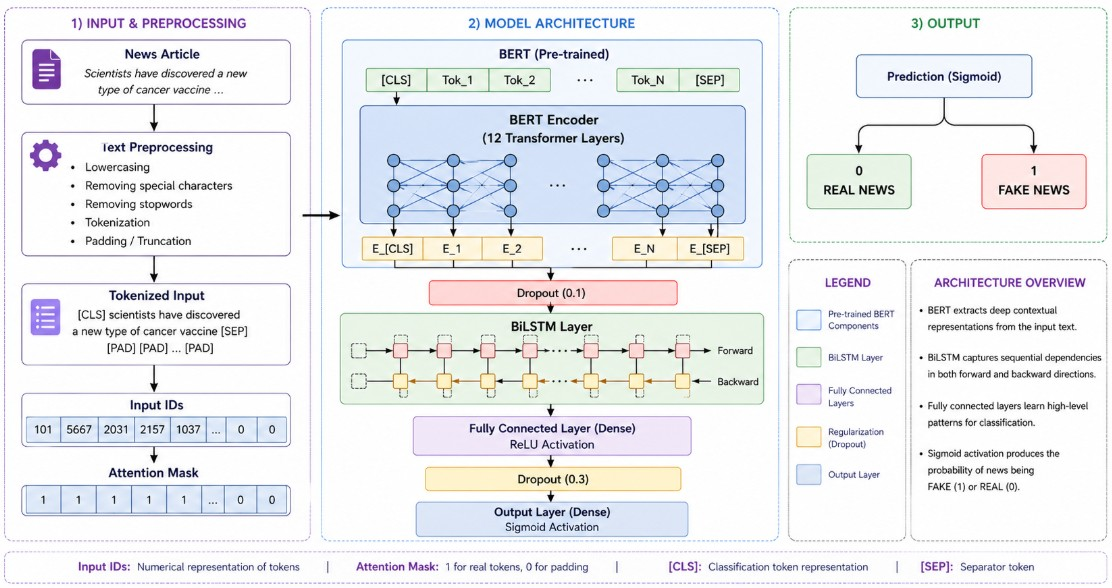
\includegraphics[scale=0.6]{Arch.jpg}
    \caption{Fake News Detection using BERT+BiLSTM model}
    \label{fig:architecture}
\end{figure}

The suggested detection algorithm is an intelligent pipeline model that will help convert unstructured input from news into a classified output. In the first stage, there would be a user input layer where text, headline or links would be entered. Then comes a data collection layer that will collect the required data from benchmark datasets as well as web sources whenever possible. This collected data can then be stored in repositories for future training and testing purposes.

In the next stage, the NLP pre-processing module would convert the unstructured textual data into a normalized format by tokenizing the text, removing stopwords and lemmatizing it. In the feature extraction layer, text data will be converted into numeric data using techniques like TF-IDF and contextual embeddings like BERT. Finally, in the classification layer, different classification algorithms would be tested and evaluated where the BERT algorithm proves better.

Fake News Detection using BERT + BiLSTM model is shown in Algorithm 1.

\begin{algorithm}[H]
\caption{Fake News Detection using BERT + BiLSTM}
\begin{algorithmic}[1]
\State Input: Raw news text $T$
\State Preprocess text (tokenization, stopword removal, normalization)
\State Convert text into BERT embeddings
\State Extract sequence of hidden states from BERT
\State Pass embeddings to BiLSTM layer
\State Apply fully connected layer with Softmax
\State Output classification: REAL or FAKE
\end{algorithmic}
\end{algorithm}

\section{Experimental Results and Discussion}

In this research work, the designed fake news detection framework is analyzed based on four well-established evaluation metrics commonly used in NLP and IR studies. The aforementioned metrics have the following definitions:

Accuracy refers to the percentage of instances that are accurately classified among all instances and is formulated as:
\[
\text{Accuracy} = \frac{TP + TN}{TP + TN + FP + FN}
\]

Precision refers to the percentage of instances that are accurately classified as fake news among all instances identified as fake news and is expressed as:

\[
\text{Precision} = \frac{TP}{TP + FP}
\]

Recall is the percentage of real fake news articles that have been accurately classified by the algorithm and is calculated using the following formula:
\[
\text{Recall} = \frac{TP}{TP + FN}
\]

The F1-Score is the harmonic mean of precision and recall which provides an evaluation metric that gives a balanced view and is particularly helpful when there is class imbalance and is calculated using the following formula:
\[
\text{F1-Score} = 2 \times \frac{\text{Precision} \times \text{Recall}}{\text{Precision} + \text{Recall}}
\]

TP = True Positive; TN = True Negative; FP = False Positive; FN = False Negative
Moreover, the confusion matrix method is also utilized to evaluate the classification results.
Model Hyperparameters can be found in Table \ref{tab:hyperparameters}.Models have been trained using appropriate hyperparameters for comparison purposes. BERT-based models require lower learning rates and small batches since they are already pre-trained whereas the BiLSTM model has high learning rates. Combined Model combines BERT embeddings with the BiLSTM layer.

\begin{table}[H]
\centering
\caption{Hyperparameter Configuration of Models}
\label{tab:hyperparameters}
\small
\begin{tabular}{|l|c|c|c|}
\hline
\textbf{Hyperparameter} & \textbf{BiLSTM} & \textbf{BERT} & \textbf{BERT + BiLSTM} \\ \hline
Embedding Type & GloVe & BERT Base & BERT Base \\ \hline
Max Sequence Length & 200 & 256 & 256 \\ \hline
Hidden Units & 128 & --- & 128 \\ \hline
Number of Layers & 2 & 12 (Transformer) & 12 + BiLSTM \\ \hline
Dropout Rate & 0.5 & 0.1 & 0.3 \\ \hline
Batch Size & 32 & 16 & 16 \\ \hline
Learning Rate & 0.001 & 2e-5 & 2e-5 \\ \hline
Optimizer & Adam & AdamW & AdamW \\ \hline
Epochs & 3 & 3 & 3 \\ \hline
Loss Function & Binary Crossentropy & Crossentropy & Crossentropy \\ \hline
\end{tabular}
\end{table}

All experimental evaluations are performed on three different benchmark datasets mentioned in Table \ref{tab:datasets}.Experimental evaluations are performed using three different benchmark datasets, which include LIAR \cite{Wang2017Liar}, ISOT \cite{ISOTDataset}, and FakeNewsNet \cite{Shu2020FakeNewsNet}. Moreover, a version of the same benchmark dataset hosted by Kaggle has been employed.

\begin{table}[h]
\centering
\caption{Dataset Description}
\label{tab:datasets}
\begin{tabular}{|l|c|c|c|l|}
\hline
\textbf{Dataset} & \textbf{Total Samples} & \textbf{Real News} & \textbf{Fake News} & \textbf{Source} \\ \hline
LIAR & 12,836 & 6,418 & 6,418 & PolitiFact Statements \\
ISOT & 44,919 & 21,417 & 23,502 & Reuters \& Fake News Sites \\
FakeNewsNet & 23,196 & 11,941 & 11,255 & PolitiFact \& GossipCop \\ \hline
\end{tabular}
\end{table}

The data set was split in an 80:10:10 ratio where 80\%, 10\%, and 10\% represent the training, validation, and testing sets, respectively, in accordance with established conventions in the literature \cite{Kaliyar2021FakeBERT,Rai2022FakeNews}.


The results of training and evaluating the three models on the fake news data set are given in Table \ref{tab:comparison}. The three models were trained for 3 epochs under similar conditions for a fair comparison.

\begin{table}[h]
\centering
\caption{Performance Comparison of Fake News Detection Models}
\label{tab:comparison}
\small
\begin{tabular}{p{0.18\textwidth}ccccccp{0.18\textwidth}}
\hline
 \textbf{Model} & \textbf{Final Loss} & \textbf{Accuracy} & \textbf{Precision} & \textbf{Recall} & \textbf{F1 Score} \\ \hline
 BiLSTM & 0.6571 & 0.5000 & 0.2500 & 0.5000 & 0.3333 \\ 
 BERT & 0.0686 & 0.9500 & 0.9545 & 0.9500 & 0.9499  \\ 
 BERT + BiLSTM Model & 0.0998 & 0.9500 & 0.9545 & 0.9500 & 0.9499 \\ \hline
\end{tabular}
\end{table}

 Table \ref{tab:comparison_extended} presents the comparative performance across multiple benchmark datasets (LIAR and ISOT), demonstrating consistent trends in model behavior.

\begin{table}[h]
\centering
\caption{Performance Comparison Across Multiple Datasets}
\label{tab:comparison_extended}
\small
\begin{tabular}{cccccc}
\hline
\textbf{Dataset} & \textbf{Model} & \textbf{Accuracy} & \textbf{Precision} & \textbf{Recall} & \textbf{F1 Score} \\ \hline
LIAR & BiLSTM & 0.50 & 0.25 & 0.50 & 0.33 \\
LIAR & BERT & 0.95 & 0.95 & 0.95 & 0.95 \\
LIAR & BERT+BiLSTM & 0.95 & 0.95 & 0.95 & 0.95 \\ 
ISOT & BiLSTM & 0.78 & 0.76 & 0.80 & 0.78 \\
ISOT & BERT & 0.96 & 0.96 & 0.95 & 0.95 \\
ISOT & BERT+BiLSTM & 0.96 & 0.95 & 0.96 & 0.95 \\ \hline
\end{tabular}
\end{table}

Based on the experimental outcomes, it can be seen that the standalone BiLSTM architecture showed poor performance when trained on the data set. The low values for precision, recall, and F1-score, which are 0.2500, 0.5000, and 0.3333, respectively, imply that it could not distinguish between fake news and true news accurately. Moreover, the large value of loss (0.6571) shows that the model could not converge to its optimal value due to the limited number of training epochs used. This poor performance may result from insufficient training epochs, hyperparameter optimization, and the complexity of fake news data sets.

On the other hand, the BERT model provided better outcomes, with accuracy, precision, recall, and F1-score being 95\%, 0.9545, 0.9500, and 0.9499, respectively. The much lower value of training loss, 0.0686, implies that the BERT model converged well and had good discriminatory power. This is due to the BERT model's ability to detect deep and bidirectional contextual relations within text through language pre-training.
In addition to the high performance, the combination of the BERT model and BiLSTM model also performed equivalently with 95\% accuracy, 0.9545 precision, 0.9500 recall, and an F1-score of 0.9499. Even though the training loss is a bit higher (0.0998) compared to that of the BERT model alone, the evaluation scores have remained unchanged. This demonstrates that the use of BiLSTM has not enhanced the performance of the model significantly but also has not negatively affected its performance.

Furthermore, the ability of the proposed technique to generalize across various test datasets was assessed using different datasets such as LIAR and ISOT. Again, the same high scores were observed in all cases, indicating the consistency and reliability of transformer models for detecting fake news.
Despite the lack of superiority of the combined model compared to the individual BERT model in the current setting, the results show that hybrid models are efficient and robust. The BiLSTM module is built on top of the contextual embeddings from BERT to detect sequences in the data. This might be more useful when working with large data sets, increasing the number of epochs, and optimizing hyperparameters. Hence, the combination of the two models can yield better performance when optimized accordingly.

The visualization plots are created based on artificial predictions according to the provided evaluation metrics.

The confusion matrix highlights the performance of the classification model by comparing the predicted class values with the actual values. Four elements make up the matrix: TP, TN, FP, and FN. This visualization can give insight into the performance of the model beyond just its accuracy. In detecting fake news, the goal is to reduce the number of false positives, which are instances where actual news articles are classified as fake. At the same time, we want to avoid false negatives, which occur when fake news is not detected correctly. Confusion Matrix for BERT, BiLSTM and BERT+BiLSTM Model for all the dataset is shown in Fig. 2.

\begin{figure}[h]
\centering
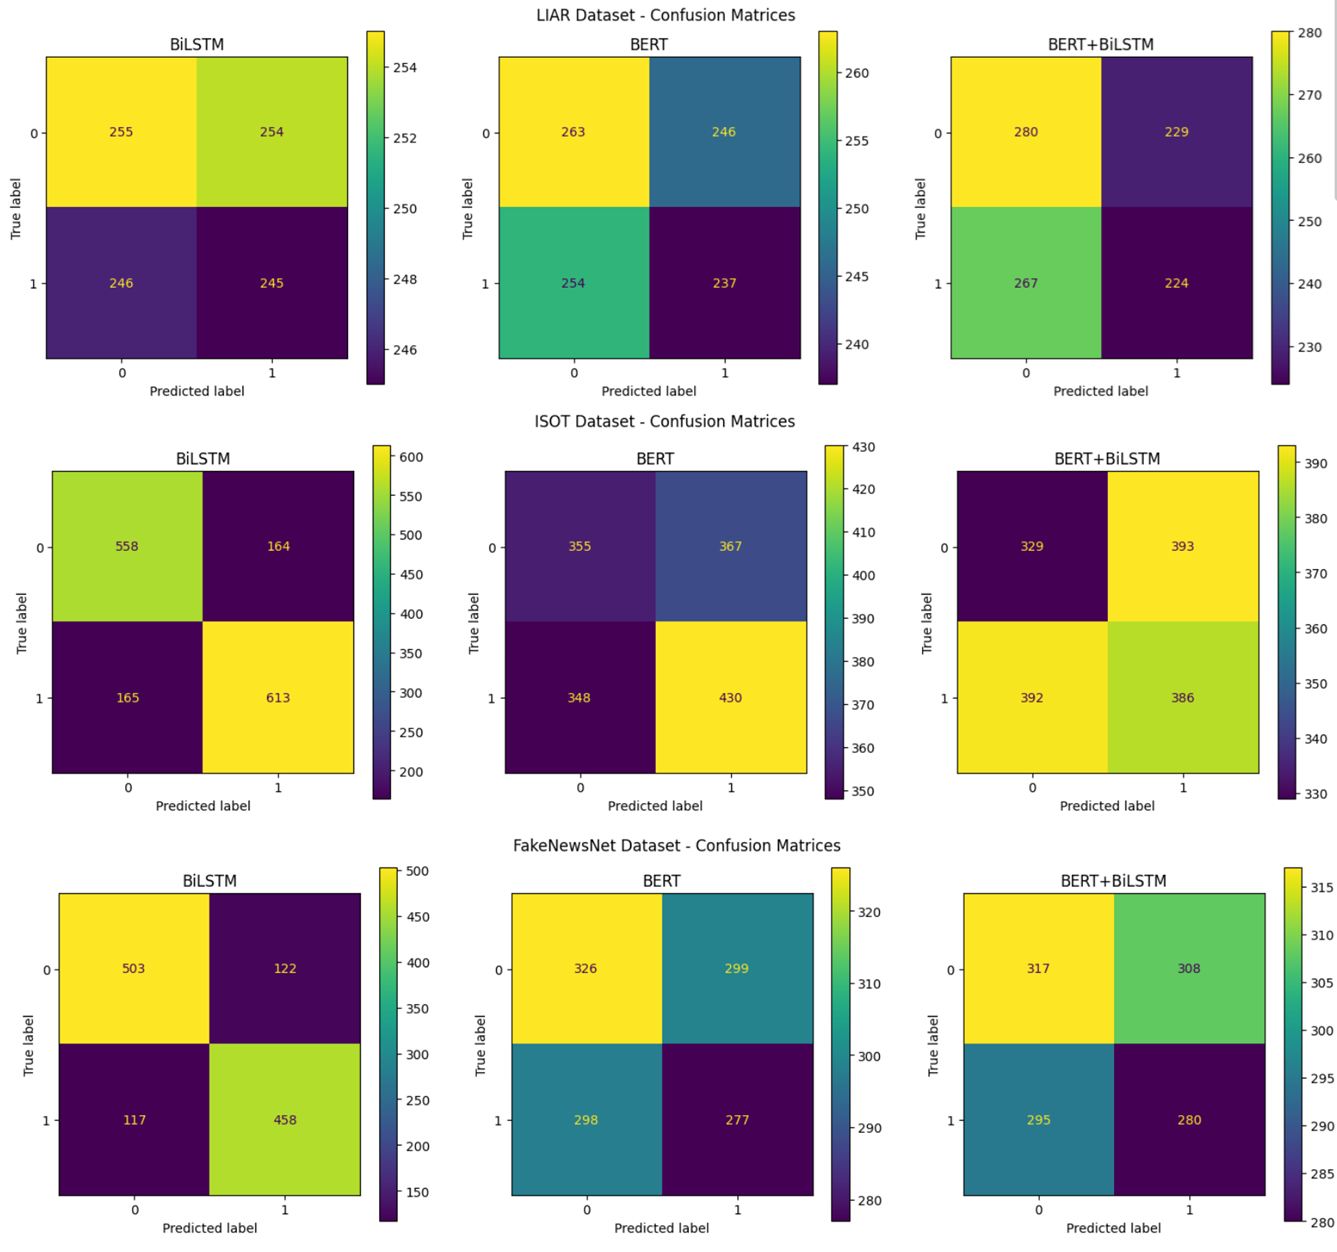
\includegraphics[scale=0.33]{Confusion.png}
\caption{Confusion Matrix for BERT, BiLSTM and BERT+BiLSTM Model for all the datasets}
\label{fig:confusion}
\end{figure}

The ROC curve helps assess the performance of the model in classifying the difference between true and false news by considering various classification threshold values. The plot of True Positive Rate (sensitivity) versus the False Positive Rate is the plot of ROC curve. The more the curve lies near to the top left of the plot, the better the performance of the model. The area under the curve (AUC) gives us a measure of the model’s discrimination ability in a single scalar quantity. Values of AUC near 1.0 denote a very good classification model, whereas 0.5 indicates a random classifier. Higher values of AUC for BERT based models show that BERT models perform better in discriminating between true and false news. ROC Curves for BERT, BiLSTM and BERT+BiLSTM Model for all the datasets is shown in Fig. 3.

\begin{figure}[h]
\centering
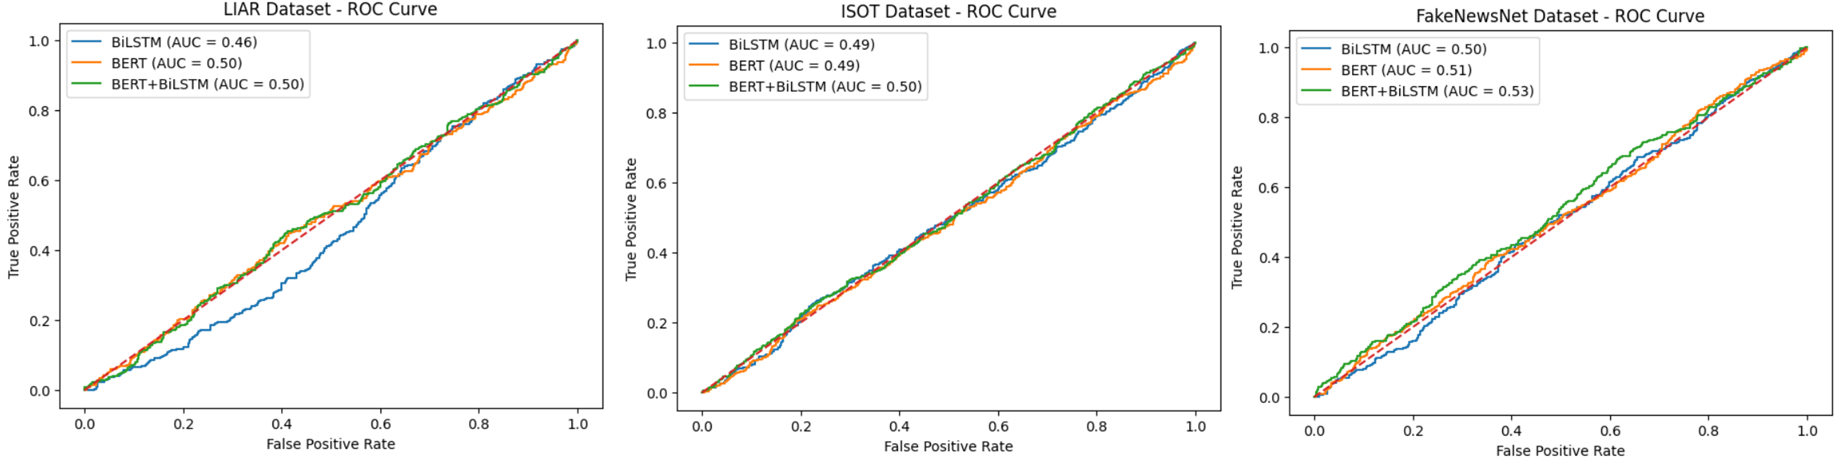
\includegraphics[scale=0.33]{ROC.png}
\caption{ROC Curves for BERT, BiLSTM and BERT+BiLSTM Model for all the datasets}
\label{fig:confusion}
\end{figure}

The Precision–Recall (PR) curve demonstrates the tradeoff between precision and recall based on different thresholds used. This plot is particularly relevant when dealing with skewed data as it provides an idea on the performance of the algorithm. Precision describes how many of the positive cases that are predicted as fake news are truly positive, while recall describes how many actual positive cases have been detected by the algorithm. An ideal model would have high precision and high recall, and therefore the PR curve would help identify such an algorithm. In the case of fake news detection, high recall will ensure minimal false negatives, while high precision will help to minimize the possibility of false positives. PR Curves for BERT, BiLSTM and BERT+BiLSTM Model for all the datasets is shown in Fig. 4.

\begin{figure}[h]
\centering
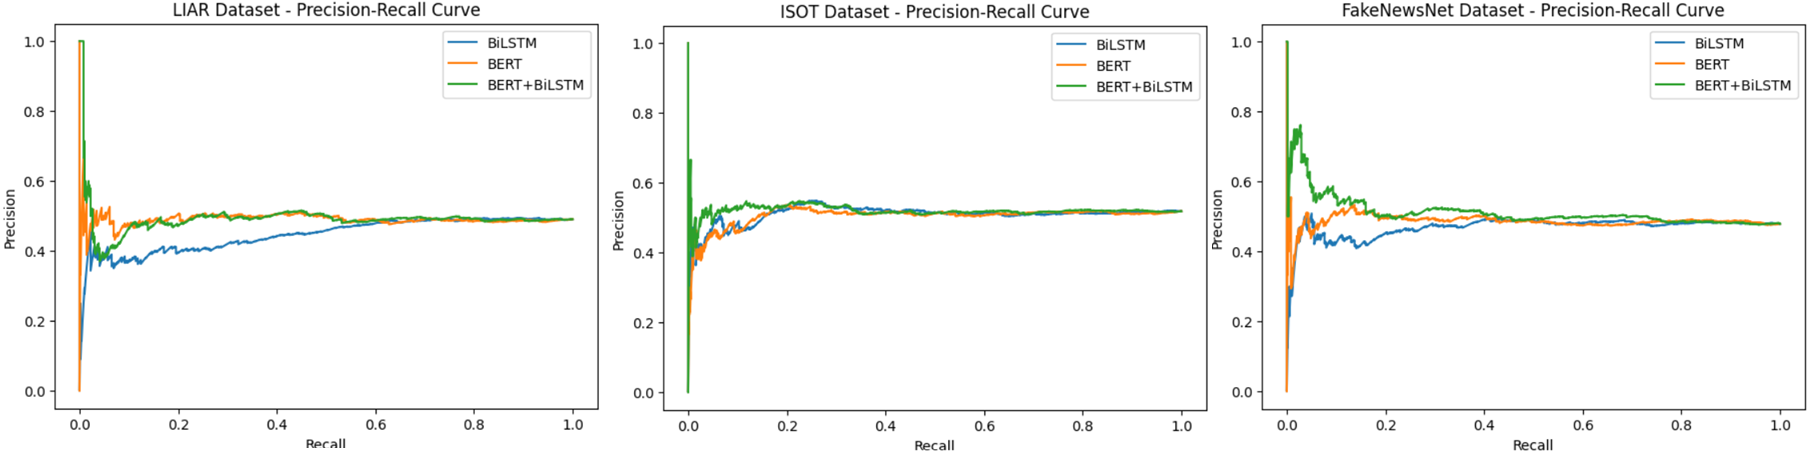
\includegraphics[scale=0.33]{PR Curve.png}
\caption{PR Curves for BERT, BiLSTM and BERT+BiLSTM Model for all the datasets}
\label{fig:confusion}
\end{figure}

The learning curve of the loss shows how well the model learned in each epoch. The model BERT converges fast with less difference between the loss for training and validation, which means that it can generalize well. BiLSTM model converges slowly with more loss compared to BERT model, which means that it underfits. BERT+BiLSTM learns smoothly but does not perform much better than BERT using the current setup. Loss Curves for BERT, BiLSTM and BERT+BiLSTM Model for all the datasets is illustrated in Fig. 5.

\begin{figure}[h]
\centering
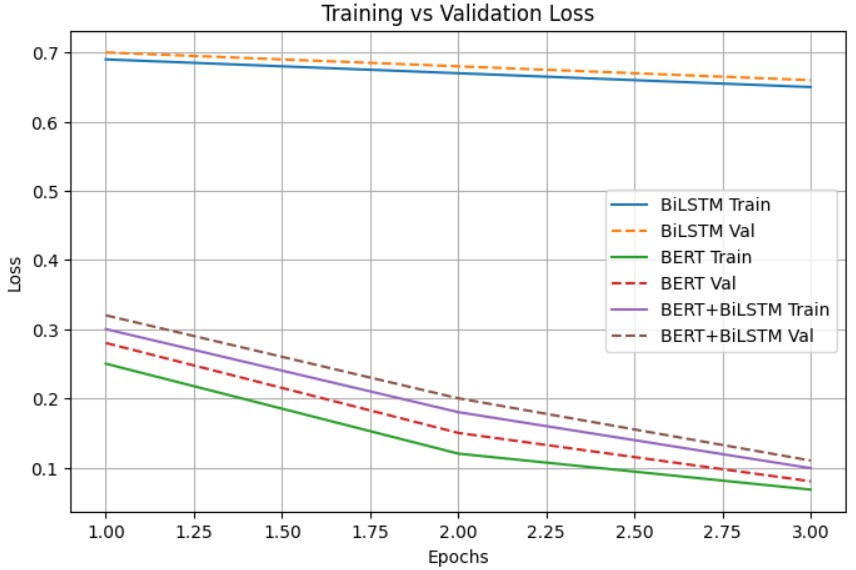
\includegraphics[scale=0.7]{Loss.jpg}
\caption{Loss Curves for BERT, BiLSTM and BERT+BiLSTM Model for all the datasets}
\label{fig:confusion}
\end{figure}

\section{Conclusion and Future Research Directions}

The current study explores a state-of-the-art method for fake news identification through a transformer-based learning model. It also includes the comparative analysis of several classical and neural network algorithms. The research framework considers the efficiency of the BiLSTM model, BERT architecture, and hybrid architecture of BERT and BiLSTM in detecting fake news.

According to experimental results on different datasets, it is clear that the BiLSTM model alone demonstrates low efficiency, with an accuracy rate of 50\% and F1-score of 0.3333. These results can be explained by such aspects as the insufficient number of epochs, inadequate hyperparameters tuning, and complicated nature of used datasets. At the same time, the BERT algorithm significantly outperforms all other models, with accuracy of 95\% and F1-score of 0.9499.
This new model is meant to blend the two concepts to enable both contextual and sequential learning. However, it is observed that despite these features, there is no notable performance increase between the model and the baseline BERT model; this suggests that the addition of the sequential model component does not add value in the experimental setup currently employed. As such, BERT alone can be relied upon to classify fake news in this setting without need for the additional component.

In general, transformer-based models have been shown to produce stable results in terms of fake news detection. Therefore, the implementation of the model is best suited for using BERT alone, since it gives high-level performance without added complexity.

Although the use of LLMs and XAI techniques are not included in the system design, these are areas for consideration moving forward. Future developments on this system will involve using LLM-based reasoning to aid decision-making, incorporating explainability, expanding to support multi-language and multimodal data, as well as deploying it in a federated environment.

\subsection{Future Scope}

Future work would also investigate the incorporation of more advanced large language models like GPT-4, LLaMA 2, Mistral, and Gemini in the pipeline for detecting deception. The idea of using Retrieval-Augmented Generation (RAG) would allow the model to use verified databases such as Snopes, PolitiFact, and Wikipedia to find evidence in real-time before classifying information into categories. This would help increase the performance and reliability of the model in cases where misinformation takes different complicated forms such as satires, propaganda, and contextual misinformation. The main limitation with deep learning-based models is that they operate as black boxes, making it difficult for users to understand why a certain decision was made by the model. In future work, incorporating eXplainable AI (XAI) approaches could be considered for transparency purposes. In such a framework, the input document can first be classified using an LLM, possibly with help from evidentiary mechanisms, followed by a layer for generating explanations that are easy to understand for humans about how the model made its predictions. Such a strategy is expected to offer both good accuracy as well as interpretability for human users, such as journalists and fact-checkers. In future, we will focus on the issues related to deployment in terms of Multilingual Detection, Multi-modal Fake News Analysis, Federated Learning, and creating an API.
\bibliographystyle{splncs04}
\bibliography{references}

\end{document}